\chapter{Architecture Dimensioning}
\label{chap:arch_dimensioning}

From the previous chapter, portions of the dataflow design space remain
undefined. Additionally, sizing of different memory banks in HERO's memory
hierarchy remain undefined. To explores what remains of the dataflow design
space this chapter introduces TEMPO. TEMPO is an optimizer for HERO templates
takes the following as an input 
\begin{itemize}
    \item A a library of networks written in pytorch
    \item A processing engine budget
    \item An objective function defined using a mixture of analytical models
    developed for estimating latency, utilization and memory access counts
\end{itemize}
From the inputs TEMPO returns the optimal PE allocation for the different
dimensions of HERO. To determine the appropriate sizes for HERO's on chip memory
(given a concrete PE allocation) CIGAR's model dim collector is used to collect
statistics on the number of elements in the different input/ output tensors of
convolution layers.  
A discussion of TEMPO's algorithm is presented in
\autoref{chap:dataflow_dse:exploring:algorithm}. The various analytical models
used to estimate power and performance metrics when running supported layers in
the TIMM library are presented in
\autoref{chap:dataflow_dse:exploring:tempo_model}. Results for different
utilization optimal configurations of HERO under various PE constraints are
presented in \autoref{chap:dataflow_dse:exploring:results}.  

\section{Exploring what remains of the dataflow design space with TEMPO}
\label{chap:dataflow_dse:exploring}

\begin{figure}[]
    \centering
    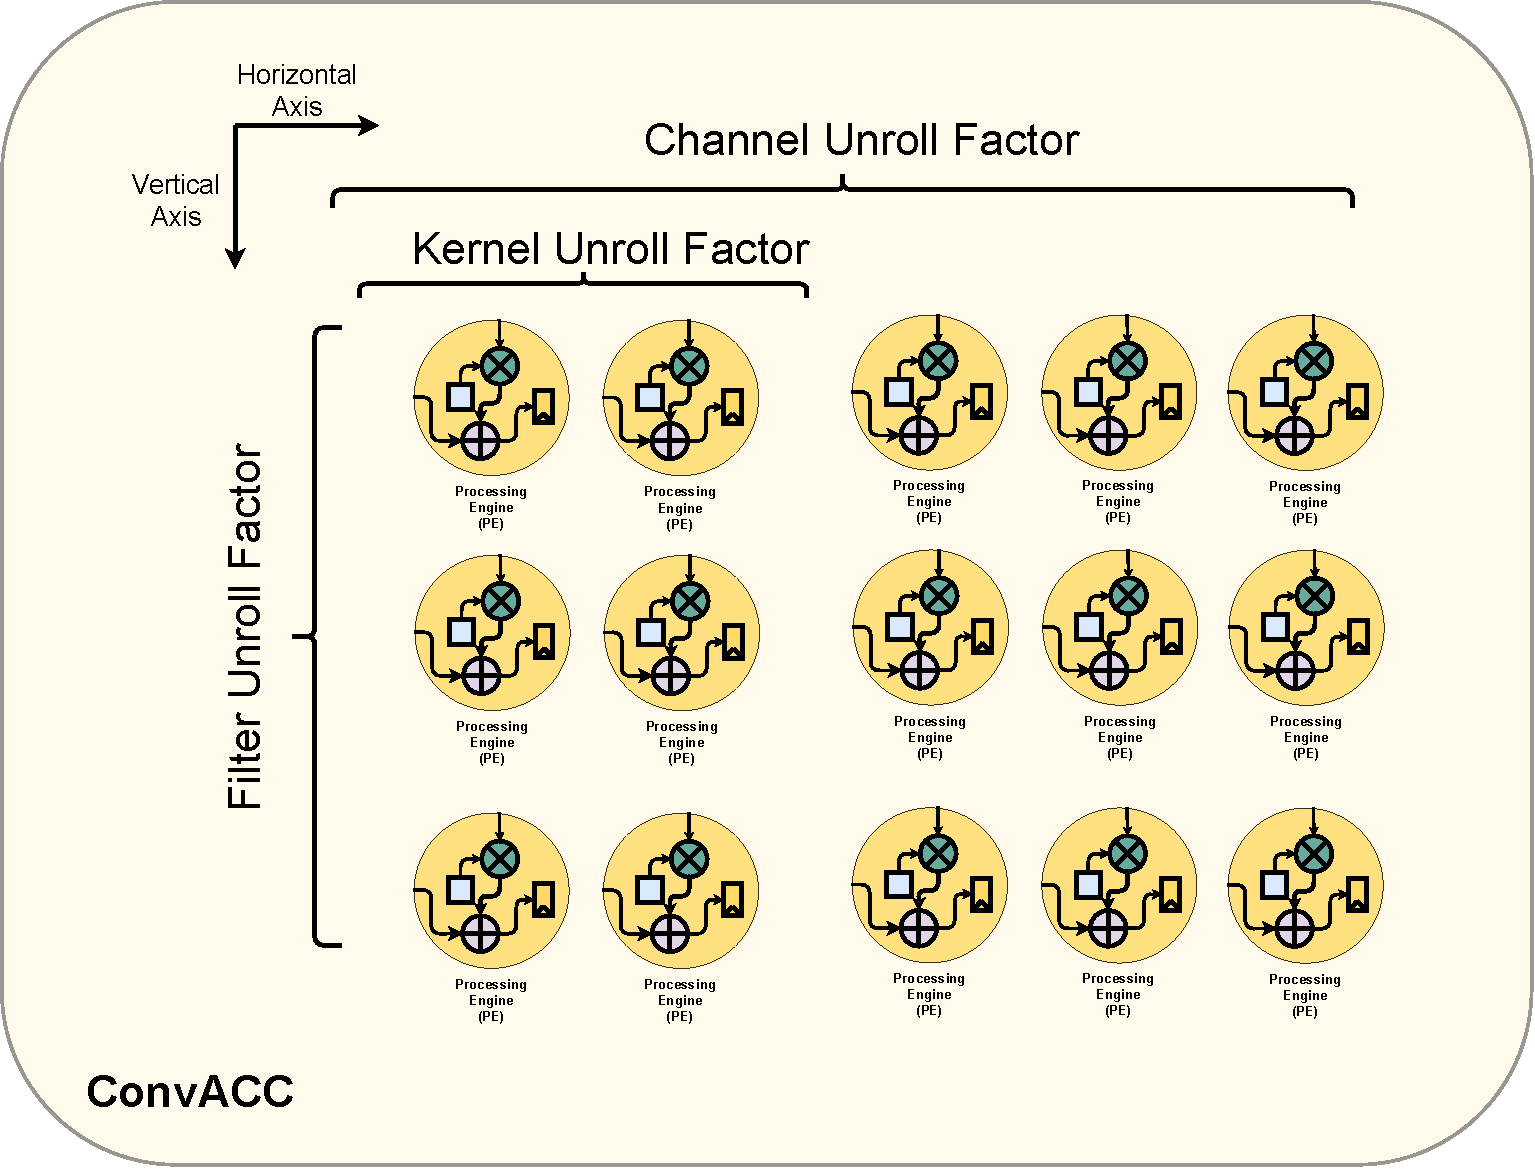
\includegraphics[scale=0.4]{fig/axis_mapping.pdf}
    \caption{\ac{GEMM} and (1, 1) Convolution Equivalence}
    \label{fig:axis_mapping}
\end{figure}

From the previous section we have concluded that loops F, C, KY and KX are all
unroll targets, and KY and KX loops should be unrolled assuming that (1, 1) and
(3, 3) kernels are supported directly. What remains of the dataflow design space
are the unroll factors for F and C loops as well as the accelerator spatial axis
mapping for all unrolled loops F, C, KY, KX. From this point these parameters
will be referred to as HERO architecture dimensions from which a concrete
accelerator instance can be defined. These accelerator architecture dimensions
define the number of processing engines allocated to process channels, filters,
and kernels concurrently in the a HERO instance. An illustration of this \ac{PE}
allocation is present in \autoref{fig:axis_mapping}. The space of possible
unroll factors is as large as the space of possible loop upper bounds for the
aforementioned unrolled loops. However, as discussed earlier, some combinations
of loop upper bounds are unlikely in real networks. Additionally, spatial axis
mapping affects the effective unroll factors when executing different
convolution layers than the ones assumed when unrolling said loops. This further
expands the design space of a possible architecture dimensions. To effectively
explore the space of loop unroll factors and accelerator spatial axis mapping we
introduce \ac{TEMPO}, a dataflow exploration and analysis tool used to optimize
an accelerator's weight stationary dataflow based on a target CNN library as
well as an arbitrary objective function. To orient the reader to TEMPO's
algorithm and analytical model first a connection is establish between loop
unrolling and tiling of the input feature map, weight and output feature map
tensors in a convolution layer in \autoref{chap:dataflow_dse:exploring:tiling}. 
Then a discussion of \ac{TEMPO}'s algorithm
model is presented in \autoref{chap:dataflow_dse:exploring:algorithm} as well as
it's analytical models for utilization, latency and access counts, in
\autoref{chap:dataflow_dse:exploring:tempo_model}. Additionally, results of
running \ac{TEMPO} on TIMMS's library of networks is presented in
\autoref{chap:dataflow_dse:exploring:results}. Finally a brief discussion on
on-chip memory hierarchy sizing will be given in
\autoref{chap:dataflow_dse:memory_hierarchy_sizing}. 


\section{Loop unrolling as a form of tiling}
\label{chap:dataflow_dse:exploring:tiling}

Depending on the chosen unroll factors of HERO, the architecture in effect tiles
the weight tensor and processes it tile by tile in the convolution operation. An
illustration of this concept is present in
\autoref{fig:tiling_connection_to_unroll_targets}. Loop unroll factors determine
PE allocation Tiling of a weight tensor arises from the processing of filters,
channels and kernels in batches whose size depend on the unroll factors. Padding
of a weight tensors is performed wherever the chosen PE binding for filter or
channel loops exceeds the number of channels and filters being processed in the
tile. In \autoref{fig:tiling_connection_to_unroll_targets} a weight tensor of
dimension $R^{6\times 3\times 2\times 2}$ is tiled with $F_{unroll} = 4$,
$C_{unroll}=8$, $K_{unroll}=2$ with kernel loops mapped to the horizontal axis
alongside channel loops. Additional padding in the horizontal and vertical axis
is added given excess allocation of PEs in both spatial axis in all tiles except
the top left one. With this representation, the accelerator processes the weight
tensors as a series of tiles to produce an output featuremap.    
This representation of the weight tensor as a series of tiles processed by the
architecture is useful when considering the scheduling of a convolution
operation in a network. Tiling of weights and their effect on scheduling is
discussed in \autoref{chap:net_compile}.

\begin{figure}[]
    \centering
    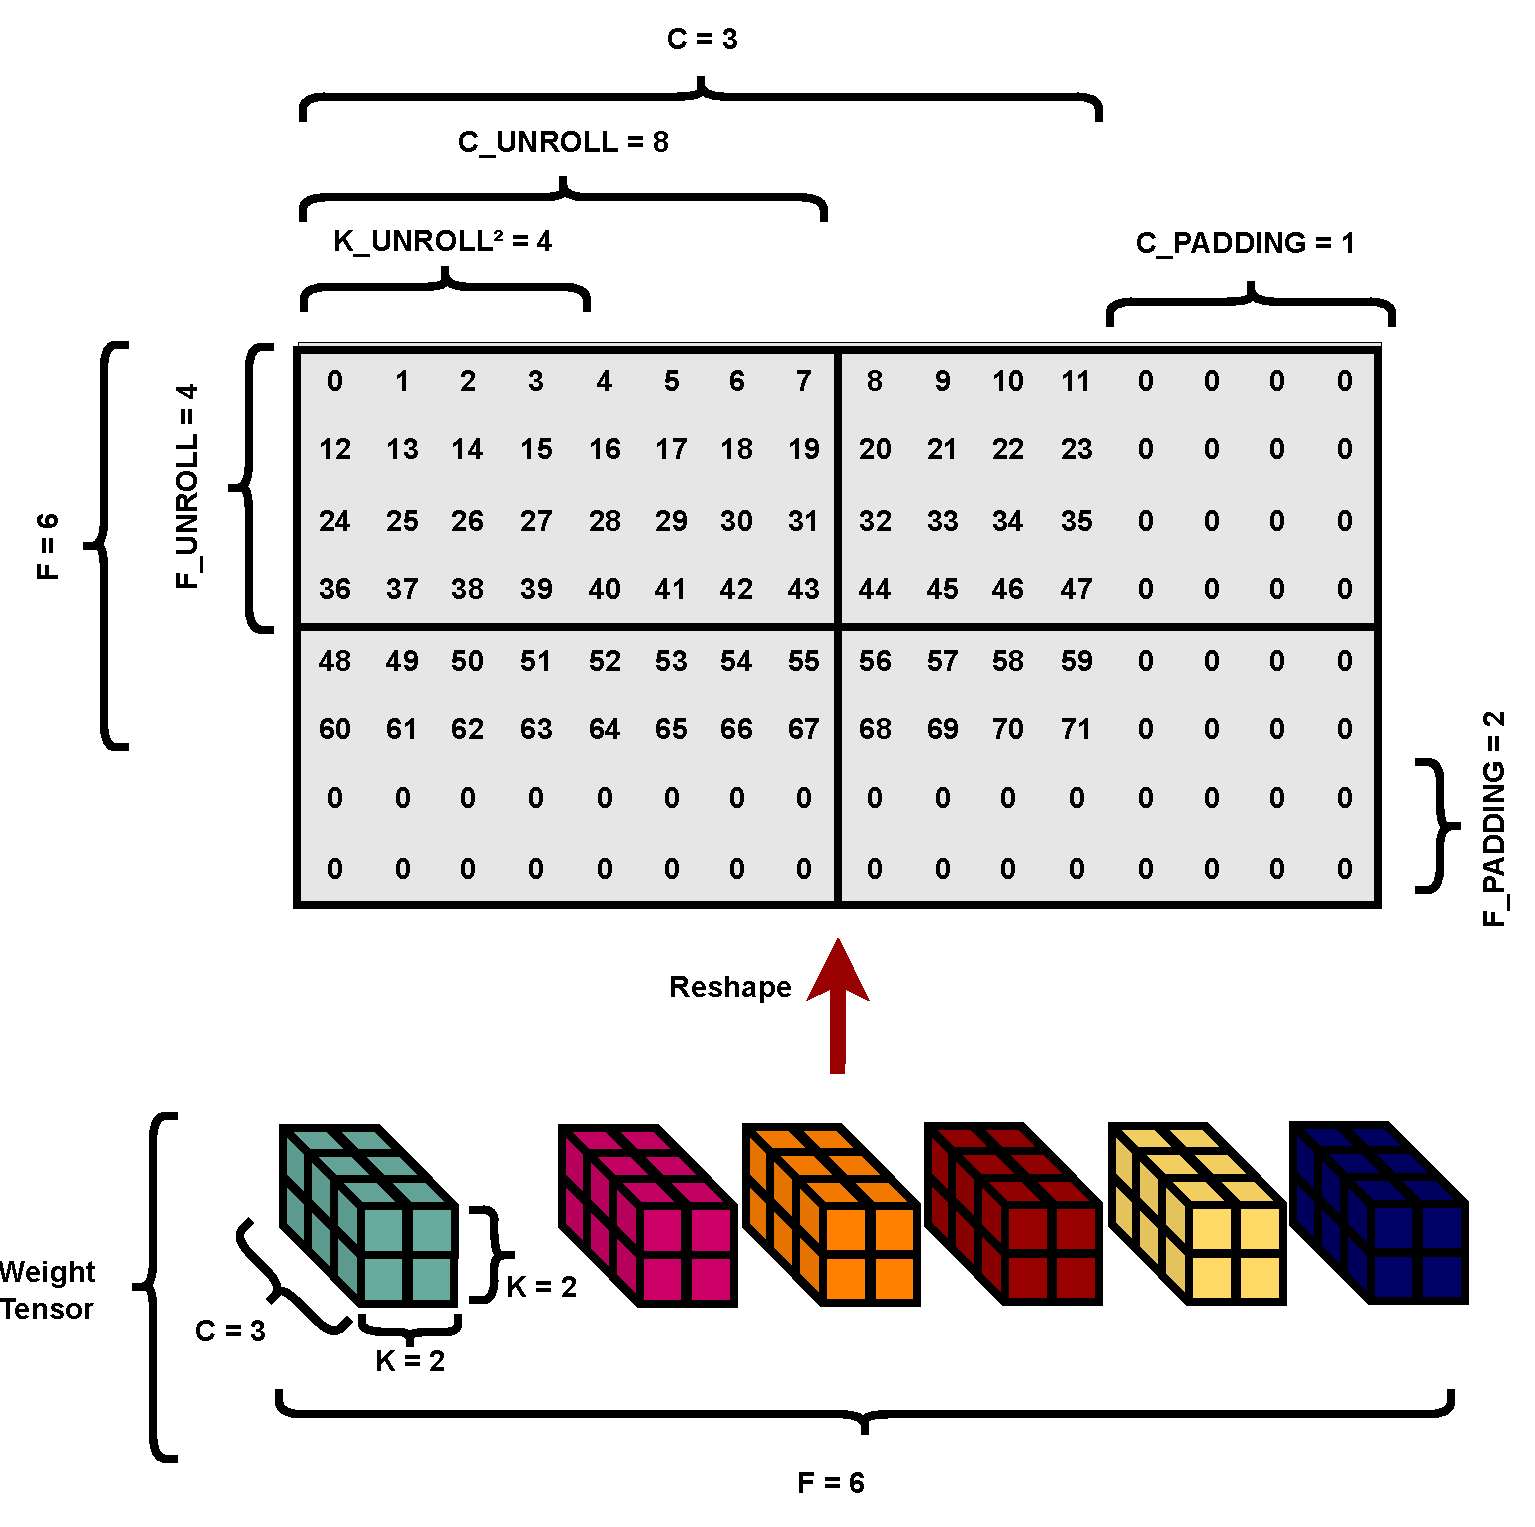
\includegraphics[scale=0.5]{fig/tiling.pdf}
    \caption{An illustration of weight tiling by loop unroll factors}
    \label{fig:tiling_connection_to_unroll_targets}
\end{figure}

\section{TEMPO Algorithm}
\label{chap:dataflow_dse:exploring:algorithm}


TEMPO's algorithm is presented in algorithm \ref{alg:tempo_algo}. TEMPO explores the
space of possible filter and channel unroll factors as well as kernel axis
mappings by exhaustively iterating through the space of possible values. TEMPO
expects the following inputs. 

\begin{itemize}
\item Processed $model^{stats}_{dict}$ from TIMM
\item An objective function $obj\_fn$
\item Maximum $pe_{budget}$ 
\item Set of kernels supported directly  $kernels_{supported}$ 
\end{itemize}

TEMPO then produces an optimal filter, channel unroll factors and kernel axis
mapping that maximizes the given objective function under the $pe_{budget}$
constraint specified. 
In algorithm \ref{alg:tempo_algo} TEMPO effectively runs an exhaustive search
using an objective function $obj\_fn$ and a set of layers from a model library.
The objective function is a function that evaluates an architectures score when
executing layers in the model library $model^{stats}_{dict}$. An architecture
score is based on any of the metrics that will be discussed in
\autoref{chap:dataflow_dse:exploring:tempo_model}. Prior to the search being
performed algorithm \ref{alg:tempo_algo} converts all layer not supported
directly in the model to (1, 1) equivalent layers based on the equivalence method
that discussed in \autoref{chap:dda:dataflow_dse:GEMM_mode}.

\begin{equation}
    \begin{aligned}
        \operatorname*{argmax}_{f_{unroll}, c_{unroll}, k_{axis}} obj\_fn(f_{unroll}, c_{unroll}, k_{axis}, ModelLibrary) \\
        \text{subject to} \\
        F_{unroll}. C_{unroll} <= Pe_{budget}
    \end{aligned}
    \label{math:tempo_algo_tldr}
\end{equation}

\begin{algorithm}[H] 
    \caption{\ac{TEMPO}}
    \label{alg:tempo_algo}
    \begin{algorithmic}[1]
    \Require{$model^{stats}_{dict}$, $obj\_fn$, $kernels_{supported}$, $pe_{budget}$} 
    \Ensure{$template^{opt}_{config}$}
    \Statex 
    \Function{TEMPO\_run}{$model^{stats}_{dict}$, $obj\_fn$, $kernels_{supported}$, $pe_{budget}$}
        \State $max_{score} \gets -\inf$
        \State $template_{opt} \gets nil$
        \State $\hat{model^{stats}_{dict}} \gets convert\_all\_unsupported\_layers(model^{stats}_{dict}, kernels_{supported})$
        \For{$f_{unroll} \gets factors(pe_{budget})$}
            \For{$k_{axis} \gets \{Verticle, Horizontal\}$}
                \State $c_{unroll} \gets \lfloor \frac{pe_{budget}}{f_{unroll}} \rfloor$ 
                \State $template_{score} \gets obj\_fn(f_{unroll}, c_{unroll}, k_{axis}, \hat{model^{stats}_{dict}})$
                \If{$max_{score} < template_{score}$}
                    \State $max_{score} \gets template_{score}$
                    \State $template_{opt} \gets template_{config}$
                \EndIf
            \EndFor
        \EndFor
        \State \Return {$template^{opt}_{config}$}
    \EndFunction
    \end{algorithmic}
\end{algorithm}

\section{TEMPO analytical model}
\label{chap:dataflow_dse:exploring:tempo_model}

On-chip memory constraints are ignored for each of the metrics evaluated using
TEMPO's analytical model. This means that TEMPO's results are the most accurate
when there are no constraints for on-chip memory. On-chip memory constraints may
limit available concurrency in a layer which will cause PEs to be underutilized.
To clarify why this happens, assume we have a convolution layer with a kernel
size of (k, k) and an ifmap of size 2 MB. Additionally, assume a single channel
of that ifmap is 512 KB. If the available on-chip ifmap memory is constrained to
512 KB the accelerator can only process one channel at a time despite the
existence of 4 channels in the ifmap tensor. If there are many PE's dedicated to
processing channels concurrently then PE utilization will suffer due to the
single channel restriction mentioned earlier. If constraints for on-chip memory
are required then an additional layer decomposition step is necessary in order
to properly evaluate all metrics that can be calculated using TEMPO's analytical
model. The inclusion of on-chip memory constraints in TEMPO's analytical model
are left as part of future work.  


% \subsection{Layer equivalence}
% \label{chap:dataflow_dse:exploring:tempo_model:layer_equivelence}

% In TEMPO's analytical model, an automatic layer conversion step is performed to
% change the dimensionality of the IFmap and Weight tensors on the basis of
% whether a layer's kernel size is supported directly or not. This conversion will
% be outlined in more detail in \autoref{chap:net_compile} which is used to extend
% support to unsupported convolution layers. Layer equivalence affects the
% dimensionality of the layers being executed on HERO and as a result it affects
% the anticipated utilization of the HERO architecture's PEs. Layer equivalence
% assumes a lowering/lifting step is performed for kernel sizes that are not (1,
% 1) and (3, 3). As discussed earlier in \autoref{chap:background:intro}, there
% are several lowering techniques available that increase the size of the ifmap
% and OFmap tensors. Of the techniques discussed is balanced lowering that aims to
% strike a balance between the memory inefficiency of lower and
% computational complexity of lowering an lifting. Balanced lowering/lifting is assumed to
% have been performed on the layers that are not directly supported by HERO.
% Lowering and lifting affect the kernel unroll factors assumed by HERO where
% unsupported layers with non (1, 1) and (3, 3) kernels are assumed to have (1, 1)
% kernel sizes  


\subsection{Utilization}
\label{chap:dataflow_dse:exploring:tempo_model:utilization}

\begin{figure}[]
    \centering
    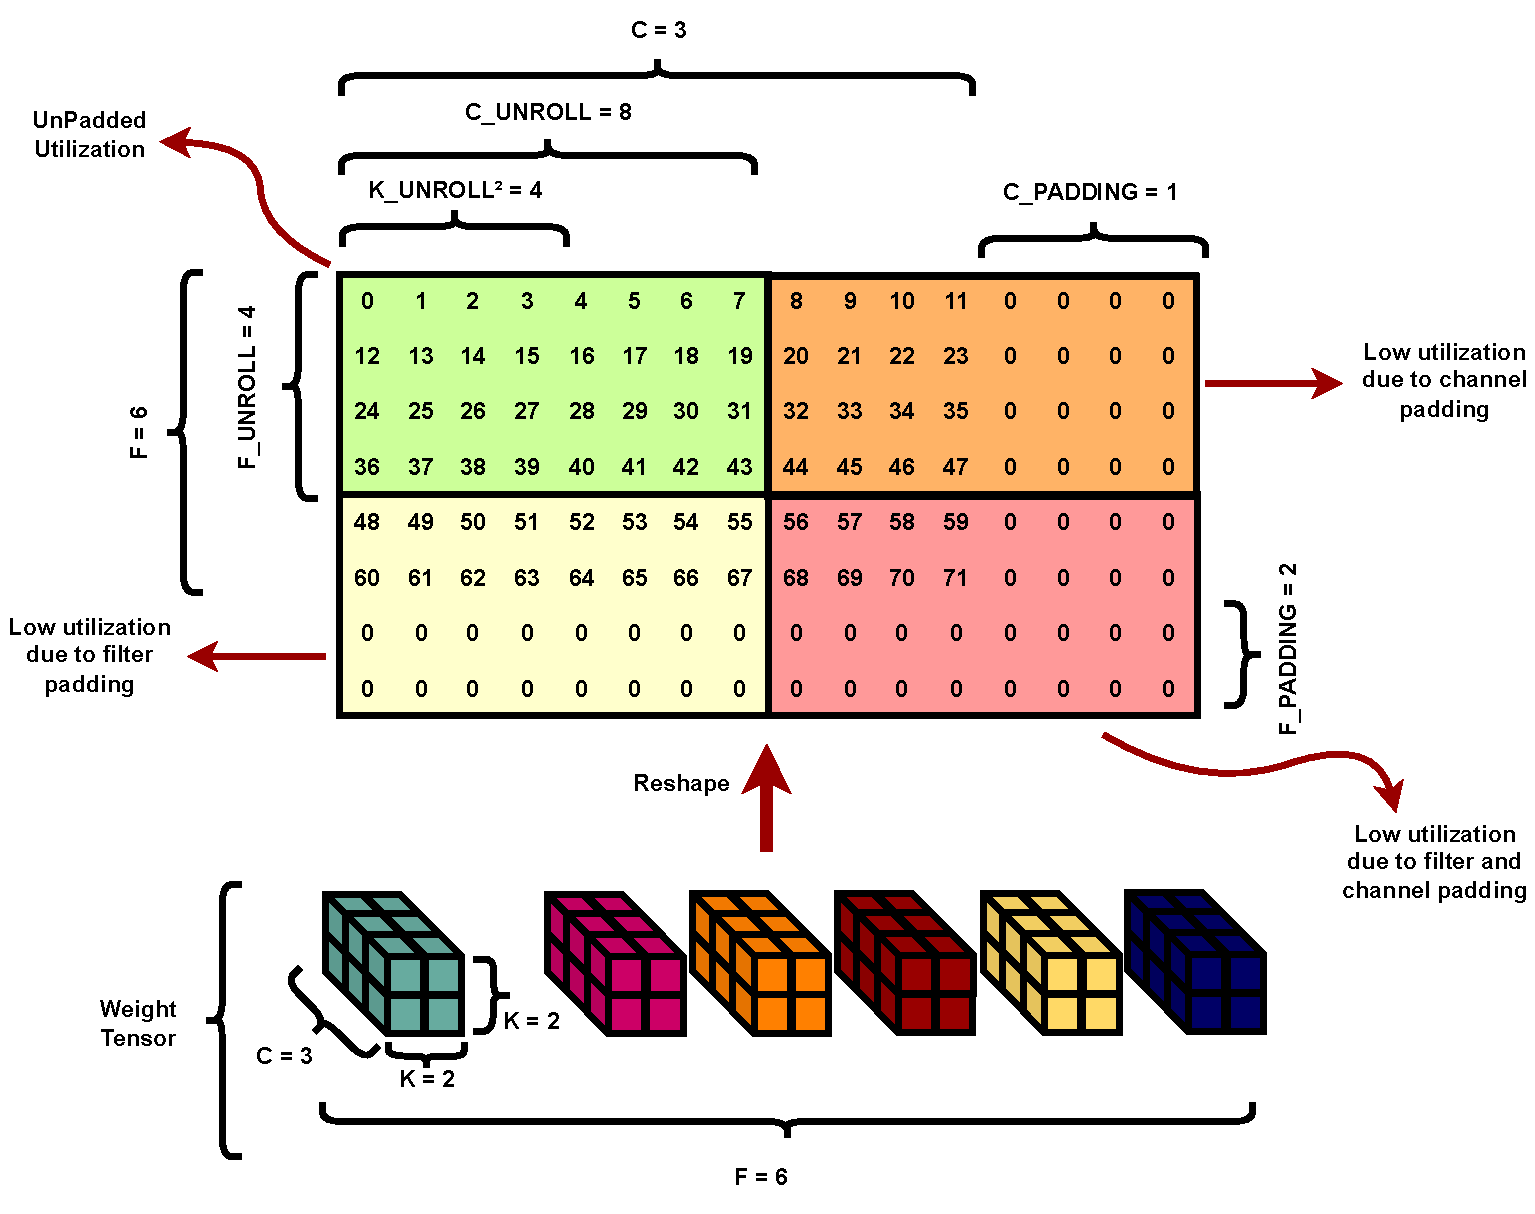
\includegraphics[scale=0.45]{fig/Lasso_ilus.pdf}
    \caption{Illustration of utilization estimation via padding analysis}
    \label{fig:tempo_model}
\end{figure}

TEMPO models accelerator utilization based on how the architecture dimensions (loop
unroll factors and loop axis mapping) tile and pad a convolution layer's
stationary weight tensor.  Kernel axis mapping is assumed to be fixed in HERO. An illustration of TEMPO's
utilization model in action is present in \autoref{fig:tempo_model}. In
\autoref{fig:tempo_model} a layer with a weight tensor of dimensionality
$R^{6\times 3\times 2\times 2}$ is tiled and padded based on the template
parameters $C_{unroll}=8$, $F_{unroll}=4$, $K_{unroll}=2$ and axis mapping
$K_{axis} = horizontal$. Based on these architecture dimensions the effective filter
and channel unroll factors are $F_{eff} = 4$, $C_{eff}=2$. These unroll factors
create $\lceil \frac{\hat{C}}{C_{eff}} \rceil = 2$ horizontal tiles and $\lceil
\frac{\hat{F}}{F_{eff}} \rceil = 2$ vertical tiles assuming padding has been
applied. The weight tensor in \autoref{fig:tempo_model} is then reshaped into a
2D matrix of dimensionality $R^{8\times 16}$ with additional padding. The total
number of tiles is then reflected in \autoref{math:total_tiles}. 

\begin{align}
    \begin{gathered}
        Count_{Tiles} = \lceil \frac{\hat{F}}{F_{eff}} \rceil \lceil \frac{\hat{C}}{C_{eff}} \rceil
        \end{gathered}
    \label{math:total_tiles}
\end{align}

Since HERO processes the weight tensor in tiles, utilization is calculated on a
per-tile basis. There are two different types of tiles, padded and unpadded,
each with their own utilization calculation. Layer utilization is then an
average of the utilizations of each tile type weighted by their frequency of
occurrence in the layer as reflect in \autoref{math:layer_utilization}. For
brevity each of the utilization equations are multiplied by their frequency of
occurrence in the same equation. 

\begin{align}
    \begin{gathered}
        LayerUtilization = \frac{utilization^{UnPadded}_{Tiles} + utilization^{Padded}_{Tile(s)}}{Count_{Tiles}} \\
            \end{gathered}
    \label{math:layer_utilization}
\end{align}

The first tile type is the unpadded tile illustrated in
\autoref{fig:tempo_model} as the green tile. Utilization is calculated using
\autoref{math:tile_utilization_unpadded}. In this tile utilization is assumed to
be 1 and it's frequency of occurrence depends on the number of unpadded tiles in
the layer $\lfloor \frac{\hat{F}}{F_{eff}} \rfloor \lfloor
\frac{\hat{C}}{C_{eff}}\rfloor$. 

\begin{align}
    \begin{gathered}
        utilization^{UnPadded}_{Tiles} = 1.\lfloor \frac{\hat{F}}{F_{eff}} \rfloor \lfloor \frac{\hat{C}}{C_{eff}}\rfloor \\
            \end{gathered}
    \label{math:tile_utilization_unpadded}
\end{align}

The second tile type is the padded tile of which there are three variations
depending on the reason for padding the tile. The utilization for all
padded tiles weighted by their frequencies of occurrence is given in
\autoref{math:unpadded_tiles_weighted_average}. 

\begin{equation}
    \begin{aligned}
        utilization^{Padded}_{Tile(s)} & = utilization^{Padded}_{ChannelTiles} \\
                                       & + utilization^{Padded}_{FilterTiles} \\
                                       & + utilization^{Padded}_{ChannelAndFilterTiles} \\
    \end{aligned}
    \label{math:unpadded_tiles_weighted_average}
\end{equation}
  
If the allocation of PEs for channel loops exceeds available channels to be
processed in the tile, then that tile will be padded. The padding in that tile results
in reduced PE utilization. An illustration of that padded tile variation is
present in \autoref{fig:tempo_model} as the orange tile.  The calculation for
the weighted utilization in that tile variation is given in equation
\autoref{math:tile_utilization_padded_channel}. To determine if a a padded channel
exists or not we can check if $\hat{C} \bmod C_{eff} > 0$ is true. If that
condition is true, padded channel tiles exist in the layer and their weighted
$utilization^{Padded}_{ChannelTiles}$ is then a function of how many PEs are
active in the tile $\frac{(\hat{C} \bmod C_{eff}) F_{eff}
K_{unroll}^2}{Count_{pe}}$ multiples by the frequency of occurrence. $\lfloor
\frac{\hat{F}}{F_{eff}} \rfloor$. If $\hat{C} \bmod C_{eff} = 0$ then there are
no padded channel tiles so $utilization^{Padded}_{ChannelTiles} = 0$.

\begin{align}
    \begin{gathered}
        utilization^{Padded}_{ChannelTiles} = \begin{cases} \frac{(\hat{C} \bmod C_{eff}) F_{eff} K_{unroll}^2}{Count_{pe}}.\lfloor \frac{\hat{F}}{F_{eff}} \rfloor
         & \hat{C} \bmod C_{eff} > 0 \\ 0
         & \hat{C} \bmod C_{eff} = 0 \end{cases} \\
            \end{gathered}
    \label{math:tile_utilization_padded_channel}
\end{align}

If the allocation of PEs for filter loops exceeds available filters to be
processed in the tile, then that tile will be padded. This another variation of
a padded tile and the weighted utilization for that tile variation is calculated
using \autoref{math:tile_utilization_padded_filter} and is illustrated in
\autoref{fig:tempo_model} as the yellow tile.

\begin{align}
    \begin{gathered}
        utilization^{Padded}_{FilterTiles} = \begin{cases} \frac{ C_{eff} (\hat{F} \bmod F_{eff}) K_{unroll}^2}{Count_{pe}}.\lfloor \frac{\hat{C}}{C_{eff}} \rfloor
            & \hat{F} \bmod F_{eff} > 0 \\ 0
            & \hat{F} \bmod F_{eff} = 0 \end{cases}
            \end{gathered}
    \label{math:tile_utilization_padded_filter}
\end{align}

Finally the last padded tile variation is the tile padded due to the excess
allocated of PEs for both filter and channel loops. This type of tile is
illustrated in \autoref{fig:tempo_model} as the red tile.  To determine if a tile like this
exists we can evaluate the condition $\hat{F} \bmod F_{eff} > 0 \land \hat{C}
\bmod C_{eff} > 0$ is true. If it there exists exactly one tile where
utilization is reduced due to excess allocation of PEs for filter and channel
loops. The equation to calculate weighted utilization in this padded tile
variation is given in \autoref{math:tile_utilization_padded_both}.

\begin{align}
    \begin{gathered}
         utilization^{Padded}_{Channel\&FilterTile} = \begin{cases} \frac{(\hat{C} \bmod C_{eff}) (\hat{F} \bmod F_{eff}) K_{unroll}^2}{Count_{pe}} & \hat{F} \bmod F_{eff} > 0 \land \hat{C} \bmod C_{eff} > 0 \\0  & else\end{cases}
            \end{gathered}
    \label{math:tile_utilization_padded_both}
\end{align}

\subsection{Latency}
\label{chap:dataflow_dse:exploring:tempo_model:latency}

Estimating latency follows the same tiling model discussed the previous
section. The latency of executing a layer based on the architecture dimensions
chosen is given in \autoref{math:latency}. Latency is a function of the number of
tiles present in the layer multiplied by the number of cycles spent processing a
single IFmap channel $\hat{Z}$ plus the additional latency incurred due to
lowering lifting depending on the support for the layer's kernel size. Latency
for lowering and lifting is given in \autoref{math:latency_lowering_lifting}. If
the kernel is supported directly, no additional lowering and lifting penalties
are incurred, otherwise penalties are calculated based on the number of
operations necessary to lower the IFmap and Weight tensors plus the number of
operations to lift the OFmap. Lowering and lifting are assumed to be performed
by a software based co-processor. The latencies associated with lowering and
lifting can be eliminated if these operations are incorporated into the processor
however, that is left as part of future work. 

\begin{align}
    \begin{gathered}
        Latency = \hat{Z}.Count_{Tiles} + Latency_{Lowering} + Latency_{Lifting} \\
                \end{gathered}
    \label{math:latency}
\end{align}

\begin{align}
    \begin{gathered}
        Latency_{Lowering} = Latency_{Lifting} = \begin{cases} 0 &  K \in \{SupportedKernels\}\\ m^{2}K & K \notin \{SupportedKernels\}\end{cases} \\
                \end{gathered}
    \label{math:latency_lowering_lifting}
\end{align}

\subsection{Memory access counts}
\label{chap:dataflow_dse:exploring:tempo_model:access_counts}

Following the tiling model discussed earlier, memory access counts are
calculated based on how the architecture dimensions tile the layer's weight tensor.
Access counts for IFmaps are given in \autoref{math:memory_access_ifmap}, OFmap
access counts are giving in \autoref{math:memory_access_OFmap} and finally
weight access counts are given in \autoref{math:memory_access_weights}.

\begin{equation}
    \begin{aligned}
        IFmap^{AccessCount} = ((\hat{Z} K_{unroll}^2) (\lfloor\frac{\hat{C}}{C_{eff}} \rfloor C_{eff} + \hat{C}\bmod C_{eff}))\lceil\frac{\hat{F}}{F_{eff}}\rceil \\
    \end{aligned}
    \label{math:memory_access_ifmap}
\end{equation}
  
\begin{equation}
    \begin{aligned}
        OFmap^{AccessCount} = 2*\hat{Z} (\lfloor\frac{\hat{F}}{F_{eff}}\rfloor F_{eff}+\hat{F}\bmod F_{eff}) \lceil\frac{\hat{C}}{C_{eff}}\rceil \\
    \end{aligned}
    \label{math:memory_access_OFmap}
\end{equation}

\begin{equation}
    \begin{aligned}
        Weight^{AccessCount} & = \hat{Z}((C_{unroll}F_{unroll})(\lfloor\frac{\hat{C}}{C_{eff}} \rfloor \lfloor\frac{\hat{F}}{F_{Feff}}\rfloor) \\
            & +(C_{unroll}F_{eff})(\lfloor\frac{\hat{C}}{C_{eff}} \rfloor \hat{F}\bmod F_{eff}) \\
            & +(C_{eff}F_{unroll})(\lfloor\frac{\hat{F}}{F_{eff}} \rfloor \hat{C}\bmod C_{eff}) \\
            & + (C_{eff}F_{eff})(\hat{F}\bmod F_{eff}\space* \hat{C}\bmod C_{eff}))
        \end{aligned}
    \label{math:memory_access_weights}
\end{equation}

\section{TEMPO results}
\label{chap:dataflow_dse:exploring:results}

\begin{equation}
    obj\_fn \gets average (\{LayerUtilization(layers)\space|\space \forall layers \in m, \forall m \in \{ModelLibrary\}\})
\label{math:tempo_results_obj_fn}
\end{equation}

Since TEMPO expects an objective function to maximize based on any or a
combination of all the discussed metrics in
\autoref{chap:dataflow_dse:exploring:tempo_model}
\autoref{math:tempo_results_obj_fn} defines an objective function based solely
on the average layer utilization metric over the entire set of convolution
layers in TIMM's model library. Layer utilization is evaluated based on the
discussion in \autoref{chap:dataflow_dse:exploring:tempo_model:utilization}.
Results for optimal configurations are given in \autoref{fig:tempo_results}.
\autoref{fig:tempo_results} shows a boxplot of average layer utilizations under
different utilization optimal configurations found with TEMPO. Median
utilization achieved for the architecture with 576 PEs was 98\% however outlier
utilization can drop to as low as 2\%. As stated earlier, TEMPO does not
consider any restrictions for on-chip memory. This may affect utilization
results due to limited available concurrency in a layer. Regardless, the
configurations suggested by TEMPO in \autoref{fig:tempo_results} without on-chip
memory constraints are a good starting point for generating results from a cycle
accurate model of HERO.


\begin{figure}[]
    \centering
    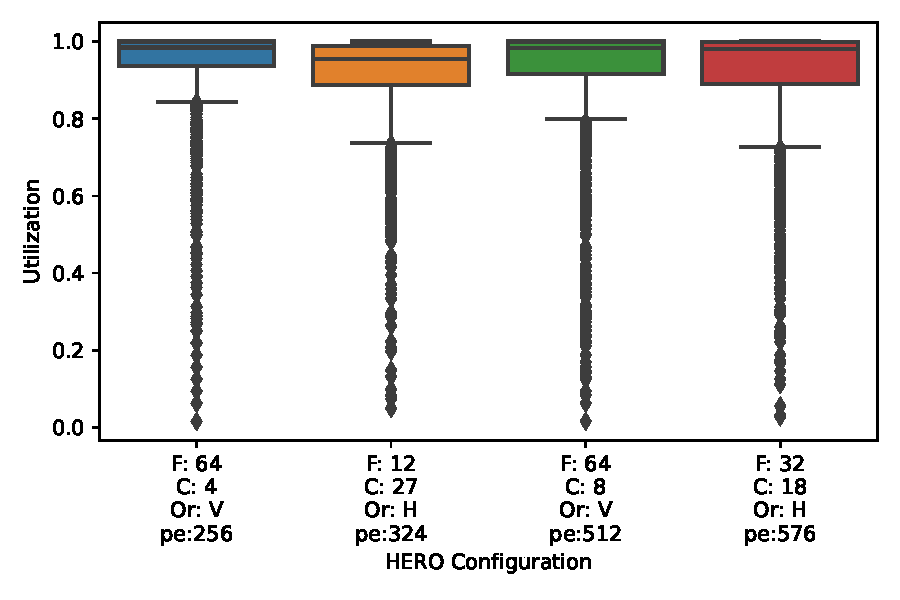
\includegraphics[scale=0.7]{Plots/tempo.pdf}
    \caption{Utilization results for different optimal configurations found using TEMPO}
    \label{fig:tempo_results}
\end{figure}


\section{Memory Hierarchy Sizing}
\label{chap:dataflow_dse:memory_hierarchy_sizing}

To determine the necessary sizes of on-chip memories we need to first look at
the sizing behavior of the different data elements in a convolution operation
(IFmaps, OFmaps and weights). Note that all discussions of storage requirements
are precision agnostic. All storage requirement results are given in number of
elements. \autoref{fig:storage:no_lowering} is a boxplot of the sizes (in number
of elements) for the storage requirements of different data element types
present in the convolution layers of the TIMM library networks. The median
storage requirements for all elements is given in \autoref{tab:median_storage}.
From both figure and table, note the similarity in storage requirements of all
data elements. Lowering and lifting operations required under GEMM mode only
increase median storage requirements by a factor of 1.01X and 1.02X for ifmap
and OFmap respectively. To support as much as 85\% of convolution layers in TIMM
without requiring layer decomposition (to be discussed in
\autoref{chap:net_compile}) we only need to allocate 1 MB of storage for IFmap
memory (L3) and OFmap memory in either of the HERO architectures presented in
\autoref{chap:dda:hw_dse:final}. Additionally since L2 storage in the ifmap
hierarchy scales with the width of ifmap tensors, it's assumed that the maximum
ifmap tensor width will not exceed 512 elements. Note that there are no storage
requirements for weight storage due to the choice of weight stationary dataflow
made in \autoref{chap:dda}. \autoref{tab:median_storage} shows the total
storage in number of elements assumed by this work. 

\begin{table}[]
    \center
    \begin{tabular}{|l|l|}
    \hline
    Data Element Type & Median Size    \\ \hline
    Weights           & $2^{16.614}$   \\ \hline
    IFmap             & $2^{16.614}$   \\ \hline
    OFmap             & $2^{16.192}$   \\ \hline
    \end{tabular}
    \caption{Table of median storage requirements for data elements in convolution layers of networks in the TIMM Library}
    \label{tab:median_storage}
\end{table}

\begin{figure}[]
    \centering
    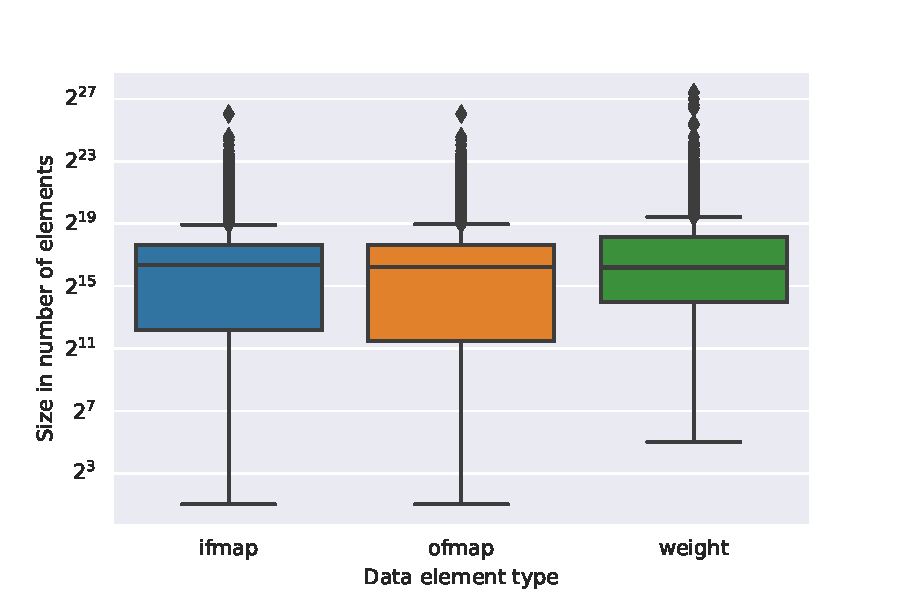
\includegraphics[scale=0.7]{Plots/storage/no_lowering.pdf}
    \caption{Boxplot of storage required for different data elements assuming no lowering}
    \label{fig:storage:no_lowering}
\end{figure}


On-chip storage requirements for IFmaps and OFmaps are influenced by the
ordering of tiles in the tiling representation of weights discussed in
\autoref{chap:dda}. The order of processing weight tiles is equivalent to the
ordering of the F, and C loops in the loop based representation of the
convolution operation discussed in \autoref{chap:dda}. Processing tiles in F, C
order (ASAP) results in retiring output featuremaps as soon as possible while retaining
input featuremaps for as long as possible. Conversely, processing tiles in C, F
order (ALAP) retains output featuremaps for as long as possible while retiring IFmaps
as soon as possible. An illustration of ASAP and ALAP tile schedules in
available in \autoref{fig:tile_scheduling}. 
% In the final template there are 4 architecture dimensions that are customizable
% depending on the target performance/area/energy efficiency requirements of the
% accelerator. The first and the second are the unroll factors for filters
% ($F_{unroll}$) and channels ($C_{unroll}$). The third is the set of directly
% supported kernels. Finally the fourth is the spatial axis mapping of the kernel
% loops ($K_{axis}$). Each of these parameters has an effect on on-chip storage
% required for the different memories accessed.

\begin{figure}
    \centering
    \subfigure[]{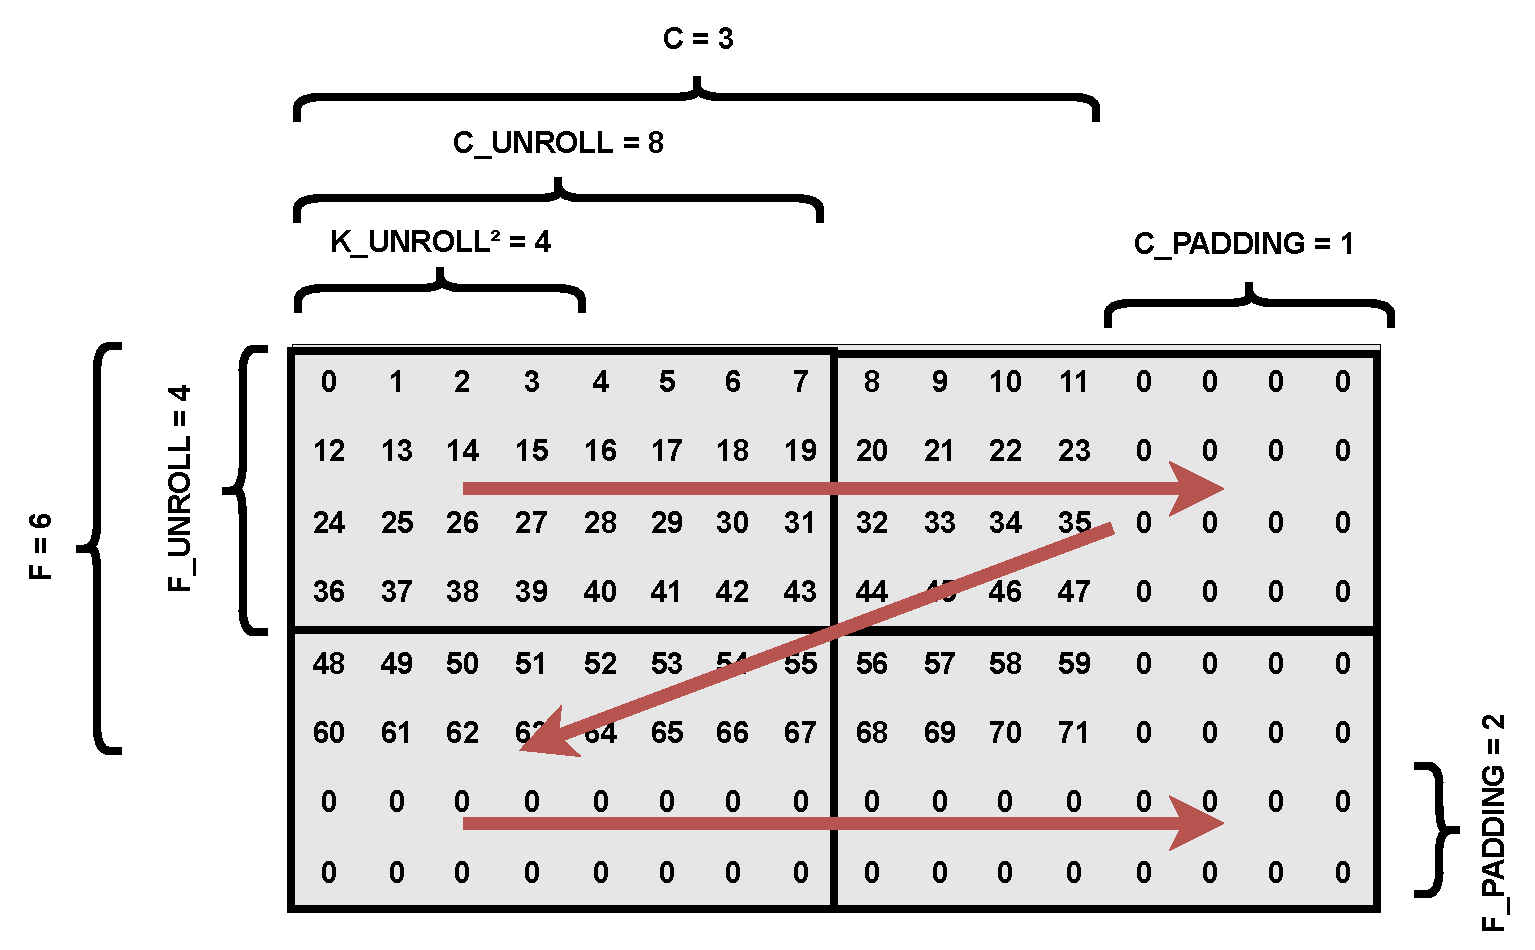
\includegraphics[width=1\textwidth]{fig/asap_tiling.pdf}}
    \hspace{0.1cm} 
    \subfigure[]{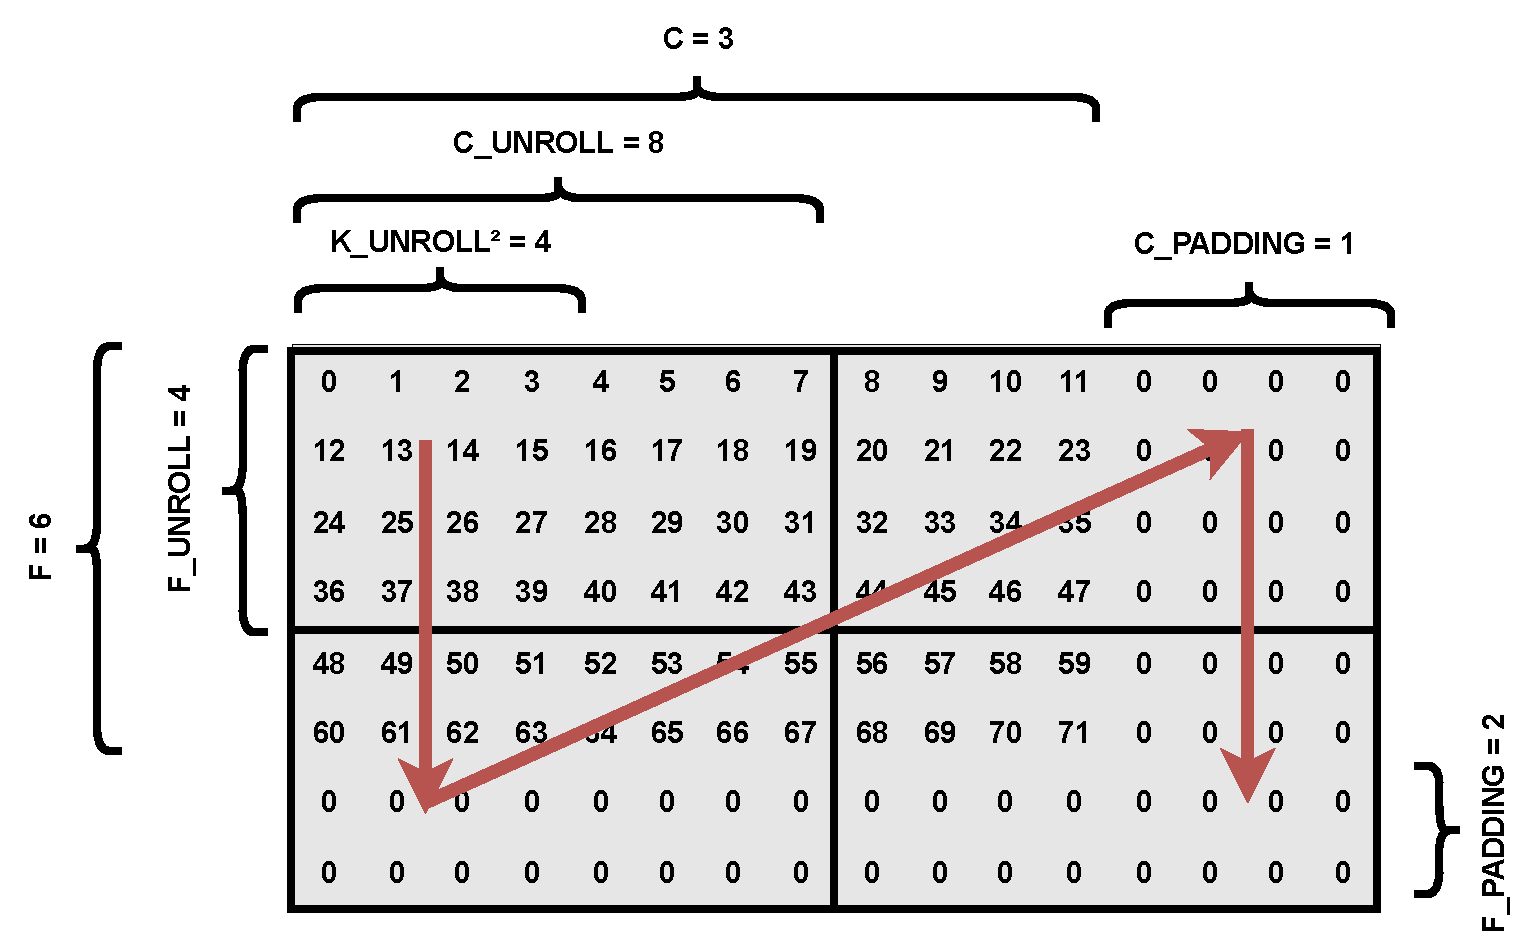
\includegraphics[width=1\textwidth]{fig/alap_tiling.pdf}}
    \caption{Illustration of different tiling schedules (a) ASAP scheduling (F, C)  (b) ALAP scheduling (C, F)}
    \label{fig:tile_scheduling}
\end{figure}

An illustration of this architectural tradeoff is present
in \autoref{fig:Fmap_scaling}.c. Note that depending on the tile scheduling
chosen, different HERO configuration parameters affect the scaling of different
on-chip memories. For example, under ASAP, input featuremap memory requirements
remain unchanged with any configuration parameters, however, OFmap memory scales
with the architecture's filter unroll factor. Under ALAP OFmap memory remains
unaffected by any of HERO's configuration parameters, however, ifmap memory scales
with the architecture's channel unroll factor. An illustration of how both
memories scale with configuration parameters is given in
\autoref{fig:Fmap_scaling}.a \& \autoref{fig:Fmap_scaling}.b. 

\begin{figure}
    \centering
    \subfigure[]{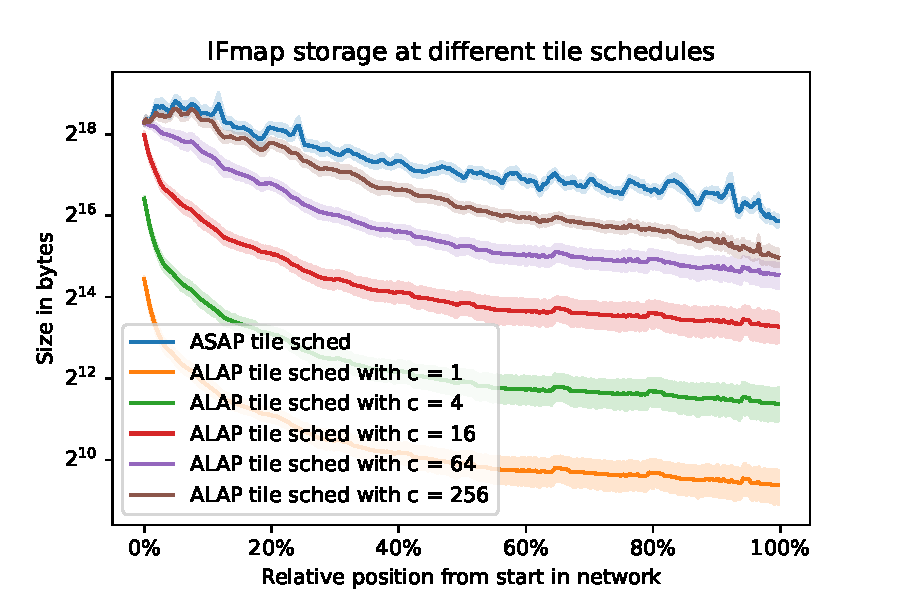
\includegraphics[width=0.45\textwidth]{Plots/ifmap_Storage.pdf}}
    \hspace{0.1cm} 
    \subfigure[]{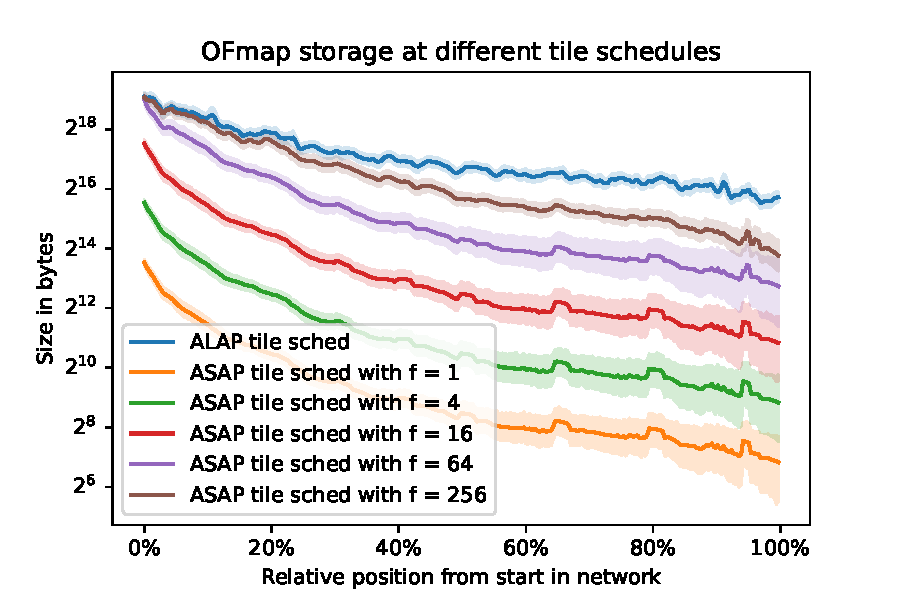
\includegraphics[width=0.45\textwidth]{Plots/PSUM_Storage.pdf}}
    \subfigure[]{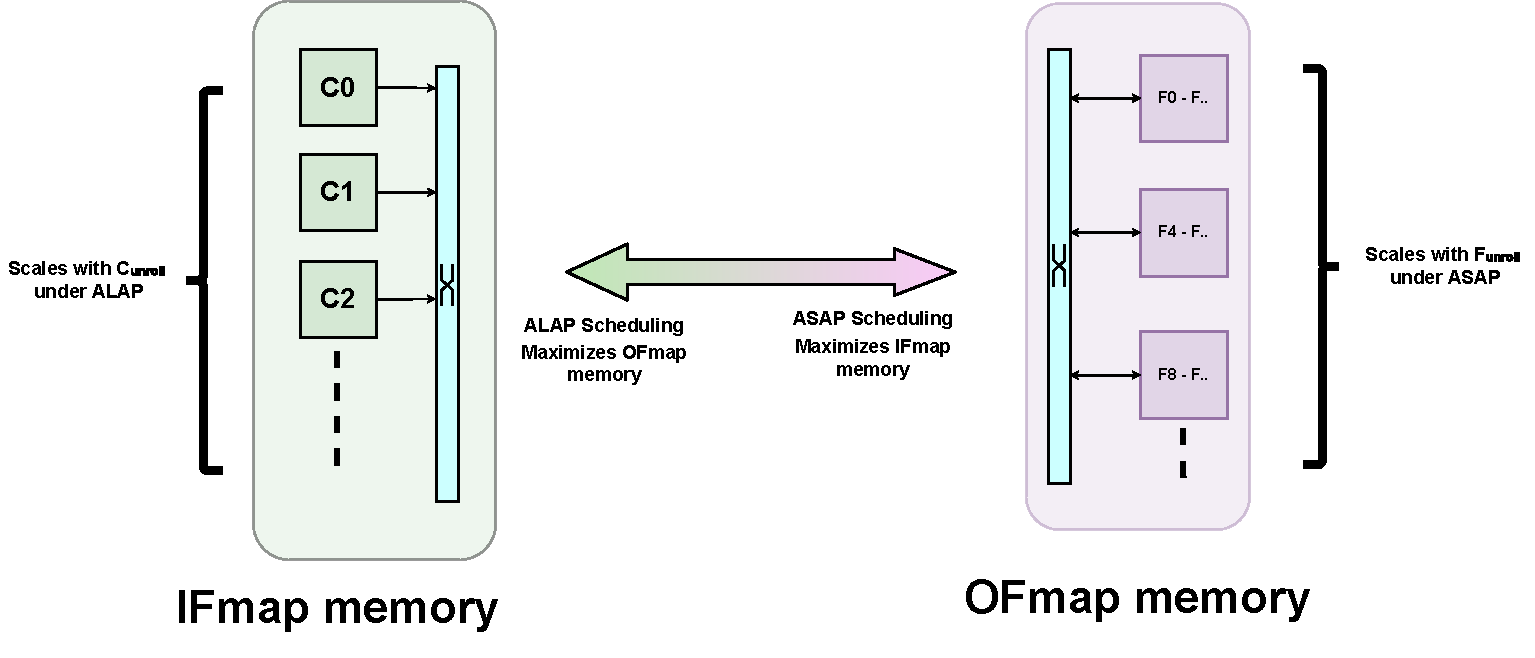
\includegraphics[width=1\textwidth]{fig/psum_ifmap_mem_scaling.pdf}}
    \caption{Illustration of storage tradeoff between OFmaps and IFmaps depending on tile scheduling (loop ordering) and accelerator configuration parameters (loop unroll factors) (a) IFmap storage (b) OFmap storage (c) architectural illustration}
    \label{fig:Fmap_scaling}
\end{figure}

In this work ASAP scheduling is always assumed given the relatively poor scaling
of OFmap memory with architecture configuration parameters. This poor scaling is due
to the necessity of storing OFmap elements using higher precision values to
prevent numeric overflow. 